\documentclass[10pt]{article}
\usepackage[T1]{fontenc}

% Document Details
\newcommand{\CLASS}{AMATH 563}
\newcommand{\assigmentnum}{Multiple Resolution Analysis}

\usepackage[margin = 1in, left=0.75in,right=0.75in]{geometry}
\usepackage{titling}
\setlength{\droptitle}{-6em}   % This is your set screw
\date{}
\renewcommand{\maketitle}{
	\clearpage
	\begingroup  
	\centering
	\LARGE \sffamily\textbf{\CLASS} \Large \assigmentnum\\[.8em]
	\large Tyler Chen\\[1em]
	\endgroup
	\thispagestyle{empty}
}
 % Title Styling


\usepackage{enumitem}

% Figures
\usepackage{subcaption}

% TikZ and Graphics
\usepackage{tikz, pgfplots}
\pgfplotsset{compat=1.12}
\usetikzlibrary{patterns,arrows}
\usepgfplotslibrary{fillbetween}

\usepackage{pdfpages}
\usepackage{adjustbox}

\usepackage{lscape}
\usepackage{titling}
\usepackage[]{hyperref}


% Header Styling
\usepackage{fancyhdr}
\pagestyle{fancy}
\lhead{\sffamily \CLASS}
\rhead{\sffamily Chen \textbf{\thepage}}
\cfoot{}

% Paragraph Styling
\setlength{\columnsep}{1cm}
\setlength{\parindent}{0pt}
\setlength{\parskip}{5pt}
\renewcommand{\baselinestretch}{1}

% TOC Styling
\usepackage{tocloft}
\iffalse
\renewcommand{\cftsecleader}{\cftdotfill{\cftdotsep}}

\renewcommand\cftchapafterpnum{\vskip6pt}
\renewcommand\cftsecafterpnum{\vskip10pt}
\renewcommand\cftsubsecafterpnum{\vskip6pt}

% Adjust sectional unit title fonts in ToC
\renewcommand{\cftchapfont}{\sffamily}
\renewcommand{\cftsecfont}{\bfseries\sffamily}
\renewcommand{\cftsecnumwidth}{2em}
\renewcommand{\cftsubsecfont}{\sffamily}
\renewcommand{\cfttoctitlefont}{\hfill\bfseries\sffamily\MakeUppercase}
\renewcommand{\cftaftertoctitle}{\hfill}

\renewcommand{\cftchappagefont}{\sffamily}
\renewcommand{\cftsecpagefont}{\bfseries\sffamily}
\renewcommand{\cftsubsecpagefont}{\sffamily}
\fi
 % General Styling
% Code Display Setup
\usepackage{listings,lstautogobble}
\usepackage{lipsum}
\usepackage{courier}
\usepackage{catchfilebetweentags}

\lstset{
	basicstyle=\small\ttfamily,
	breaklines=true, 
	frame = single,
	rangeprefix=,
	rangesuffix=,
	includerangemarker=false,
	autogobble = true
}


\usepackage{algorithmicx}
\usepackage{algpseudocode}

\newcommand{\To}{\textbf{to}~}
\newcommand{\DownTo}{\textbf{downto}~}
\renewcommand{\algorithmicdo}{\hspace{-.2em}\textbf{:}}
 % Code Display Setup
% AMS MATH Styling
\usepackage{amsmath, amssymb}
\newcommand{\qed}{\hfill\(\square\)}

%\newtheorem*{lemma}{Lemma} 
%\newtheorem*{theorem}{Theorem}
%\newtheorem*{definition}{Definition}
%\newtheorem*{prop}{Proposition}
%\renewenvironment{proof}{{\bfseries Proof.}}{}


% mathcal
\newcommand{\cA}{\ensuremath{\mathcal{A}}}
\newcommand{\cB}{\ensuremath{\mathcal{B}}}
\newcommand{\cC}{\ensuremath{\mathcal{C}}}
\newcommand{\cD}{\ensuremath{\mathcal{D}}}
\newcommand{\cE}{\ensuremath{\mathcal{E}}}
\newcommand{\cF}{\ensuremath{\mathcal{F}}}
\newcommand{\cG}{\ensuremath{\mathcal{G}}}
\newcommand{\cH}{\ensuremath{\mathcal{H}}}
\newcommand{\cI}{\ensuremath{\mathcal{I}}}
\newcommand{\cJ}{\ensuremath{\mathcal{J}}}
\newcommand{\cK}{\ensuremath{\mathcal{K}}}
\newcommand{\cL}{\ensuremath{\mathcal{L}}}
\newcommand{\cM}{\ensuremath{\mathcal{M}}}
\newcommand{\cN}{\ensuremath{\mathcal{N}}}
\newcommand{\cO}{\ensuremath{\mathcal{O}}}
\newcommand{\cP}{\ensuremath{\mathcal{P}}}
\newcommand{\cQ}{\ensuremath{\mathcal{Q}}}
\newcommand{\cR}{\ensuremath{\mathcal{R}}}
\newcommand{\cS}{\ensuremath{\mathcal{S}}}
\newcommand{\cT}{\ensuremath{\mathcal{T}}}
\newcommand{\cU}{\ensuremath{\mathcal{U}}}
\newcommand{\cV}{\ensuremath{\mathcal{V}}}
\newcommand{\cW}{\ensuremath{\mathcal{W}}}
\newcommand{\cX}{\ensuremath{\mathcal{X}}}
\newcommand{\cY}{\ensuremath{\mathcal{Y}}}
\newcommand{\cZ}{\ensuremath{\mathcal{Z}}}

% mathbb
\usepackage{bbm}
\newcommand{\bOne}{\ensuremath{\mathbbm{1}}}

\newcommand{\bA}{\ensuremath{\mathbb{A}}}
\newcommand{\bB}{\ensuremath{\mathbb{B}}}
\newcommand{\bC}{\ensuremath{\mathbb{C}}}
\newcommand{\bD}{\ensuremath{\mathbb{D}}}
\newcommand{\bE}{\ensuremath{\mathbb{E}}}
\newcommand{\bF}{\ensuremath{\mathbb{F}}}
\newcommand{\bG}{\ensuremath{\mathbb{G}}}
\newcommand{\bH}{\ensuremath{\mathbb{H}}}
\newcommand{\bI}{\ensuremath{\mathbb{I}}}
\newcommand{\bJ}{\ensuremath{\mathbb{J}}}
\newcommand{\bK}{\ensuremath{\mathbb{K}}}
\newcommand{\bL}{\ensuremath{\mathbb{L}}}
\newcommand{\bM}{\ensuremath{\mathbb{M}}}
\newcommand{\bN}{\ensuremath{\mathbb{N}}}
\newcommand{\bO}{\ensuremath{\mathbb{O}}}
\newcommand{\bP}{\ensuremath{\mathbb{P}}}
\newcommand{\bQ}{\ensuremath{\mathbb{Q}}}
\newcommand{\bR}{\ensuremath{\mathbb{R}}}
\newcommand{\bS}{\ensuremath{\mathbb{S}}}
\newcommand{\bT}{\ensuremath{\mathbb{T}}}
\newcommand{\bU}{\ensuremath{\mathbb{U}}}
\newcommand{\bV}{\ensuremath{\mathbb{V}}}
\newcommand{\bW}{\ensuremath{\mathbb{W}}}
\newcommand{\bX}{\ensuremath{\mathbb{X}}}
\newcommand{\bY}{\ensuremath{\mathbb{Y}}}
\newcommand{\bZ}{\ensuremath{\mathbb{Z}}}

% alternative mathbb
\newcommand{\NN}{\ensuremath{\mathbb{N}}}
\newcommand{\RR}{\ensuremath{\mathbb{R}}}
\newcommand{\CC}{\ensuremath{\mathbb{C}}}
\newcommand{\ZZ}{\ensuremath{\mathbb{Z}}}
\newcommand{\EE}{\ensuremath{\mathbb{E}}}
\newcommand{\PP}{\ensuremath{\mathbb{P}}}
\newcommand{\VV}{\ensuremath{\mathbb{V}}}
\newcommand{\cov}{\ensuremath{\text{Co}\VV}}
% Math Commands

\newcommand{\st}{~\big|~}
\newcommand{\stt}{\text{ st. }}
\newcommand{\ift}{\text{ if }}
\newcommand{\thent}{\text{ then }}
\newcommand{\owt}{\text{ otherwise }}

\newcommand{\norm}[1]{\left\lVert#1\right\rVert}
\newcommand{\snorm}[1]{\lVert#1\rVert}
\newcommand{\ip}[1]{\ensuremath{\left\langle #1 \right\rangle}}
\newcommand{\pp}[3][]{\frac{\partial^{#1}#2}{\partial #3^{#1}}}
\newcommand{\dd}[3][]{\frac{\d^{#1}#2}{\d #3^{#1}}}
\renewcommand{\d}{\ensuremath{\mathrm{d}}}

\newcommand{\indep}{\rotatebox[origin=c]{90}{$\models$}}




 % Math shortcuts

\usepackage{dblfloatfix}    % To enable figures at the bottom of page

% Problem
\newenvironment{problem}[1]{\vspace{2em}{\large\sffamily\textbf{#1}}\itshape\par}{}

\usepackage{nameref}
\newcommand{\vln}{\rotatebox{90}{--}}

\begin{document}

\twocolumn[{%
\begin{@twocolumnfalse}
\maketitle
\vspace{2em}
\begin{abstract}
We introduce Multiple Resolution Analysis and the Discrete Wavelet Transform. We then discuss how these might be applied to a data set of global ocean temperatures over the past few decades in order to isolate El Ni\~no. We find that the Oceanic Ni\~no Index can be recovered using just a single spatial point. Finally, we train a neural net to predict the next time the ONI will reach a certain value.
\end{abstract}

\vspace{4em}
%\tableofcontents
%\vspace{3em}
\pagebreak\end{@twocolumnfalse}
}]

\section{Introduction and Overview}
Multiple Resolution Analysis (MRA) provides a way to view data on multiple scales in both the position and frequency domains simultaneously.

The El Ni\~no Southern Oscillator (ENSO) is an ``irregularly periodic varaition in winds and sea surface temperatures over the tropical easter Pacific Ocean''. The warm phase is referred to as El Ni\~no and the cold phase is referred to as La Ni\~na. When the ENSO is at its extremes, there is often extreme weather throughout part of the world.

We apply MRA to a ocean surface temperature data set in the hopes of extracting information useful in predicting El Ni\~no.

\section{Theoretical Background}


\subsection{Multiple Resolution Analysis (MRA)}
Broadly, Multiple Resolution Analysis provides a way to obtain information at multiple scales (as the name suggests). We illustrate this with an example.

Suppose we have an audio recording of a piano. The recording tells us the amplitude of the sounds waves at a given time. What if we want to know which notes were played? We could take the Fourier transform of our recording and get information about the frequencies present. However, unless the notes were played through the entire recording, this would not be very useful.

Multiple resolution analysis lets us get information about what notes were played when. Low frequencies, which have periods comparable to the entire recording can be extracted, but without timing information, while high frequencies can be pinpointed in time. This example illustrates the basic principle of MRA.


\begin{figure*}[h]\centering
\foreach \i in {0,...,7}{
\begin{subfigure}{.24\textwidth}\centering
\includegraphics[width=\textwidth]{img/haar/basis_\i.pdf}
\end{subfigure}
}
\caption{Haar basis with \( N=8 \)}
\label{haar}
\end{figure*}

\subsection{Discrete Wavelet Transform}
One way to get time frequency information is to split the data into many pieces and take the Fourier transform of each piece. This would tell us information about which frequencies are present, as well as when these frequencies are present. Such a decomposition is often referred to as a spectogram or Short Time Discrete Fourier Transform (STDFT).

In the discrete case it is easy to see that such a transform is just a change of basis. Figure~\ref{haar} shows a possible basis for \( \RR^8 \). This basis gives us information about 4 different frequencies, as well as information about where these frequencies occur in time.

From this figure it is obvious that these functions are orthogonal, and could be appropriately normalized. It is also clear that such a basis can be generalized to any \( 2^k \)-dimensional vectorspace over \( \RR \). This basis has some advantages over a STDFT, namely that it is able to pick up low frequency modes which have a period longer than the windows in a STDFT.

This approach can be generalized to to a a class of transforms commonly referred to as the Discrete Wavelet Transform. While we show only a class of ``wavelets'' calleed ``Haar Wavelets'', many other shapes can be used. Note that the same ``wavelet'' seen in the first non-constant mode is just shifted and scaled to produce an orthonormal basis. Therefore it should not be surprising that there are many possible wavelets which are used in practice.

Like the Discrete Fourier Transform, there are efficient algorithms for computing the DWT for many wavelets.

Such a transform can be applied to vector-spaces where the vectors are multi-dimensional arrays (for instance a photo).
More specifically, suppose our data lives in \( \RR^{k_1\times k_2\times\cdots\times k_d} \).

Let \( \mB_i = \{b_{i1},b_{i2},\ldots, b_{ik_i}\} \) be a wavelet basis for \( \RR^{k_i} \). Then,
\begin{align}
    \mB = \mB_1\otimes \mB_2 \otimes \cdots \otimes \mB_d
\end{align}
is a basis for \( \RR^{k_1\times k_2\times\cdots\times k_d} \), where \( \otimes \) denotes the tensor product. In the 2-dimensional case this is simply the collection of all possible outer products of the elements of the bases for each dimension.

Such a change of basis would give information about the position and frequency/wave number of the data in each dimension. For instance, as discussed later, information about the location of a ocean temperate event in both space (longitude and latitude) and time along with information about frequency (in both spatial dimensions and in time) can be gathered.

Such a change of basis is not practical to compute for an arbitrary wavelet basis using naive algorithms since the dimension of the vector-space would generally be quite large. In particular, computing the standard inner product of two vectors of size \( N \) requires \( \mO(2N) \) operations. Even if these vectors can be accessed in constant time, a change of basis would require \( N \) inner products to project the data onto each of the \( N \) new basis vectors. Therefore it will require something like \( \mO(N^2) \) operations to compute the change of basis. With vectors with millions of components this is not practical.

There are almost certainly better algorithms for certain bases to help deal with this problem.

\subsection{SVD}
We can also perform MRA using the SVD.

Given any vector of the size of a single snapshot of our data we can project our data onto this vector and see how this ``mode'' varies in time. That means, if we are able to isolate a vector which represents El Ni\~no we would be able to see hot his varies in time.

\subsection{Filtering}
Filtering is a common technique in signal processing where the frequency content of a signal is altered. A low pass filter maintains the low frequencies of a signal and attenuates the high frequencies of a signal. This can be useful for de-noising a signal or removing a high frequency periodic piece of a signal.

\subsection{Oceanic Ni\~no Index}

The Oceanic Ni\~no Index (ONI) is a 3 month running mean of ERSST.v5 SST anomalies in the Ni\~no 3.4 region (5\( ^\circ \)N-5\( ^\circ \)S, 120\( ^\circ \)-170\( ^\circ \)W) \cite{oni}. This gives a measure of El Ni\~no events.

\begin{figure*}[bh]\centering
\foreach \j in {0,...,7}{
\begin{subfigure}{.24\textwidth}\centering
\includegraphics[width=\textwidth]{img/svd/1455/u_\j.pdf}
\end{subfigure}
}
\caption{First 8 modes of SVD of full data (all with same color scale)}
\label{full_svd_u}
\end{figure*}

\begin{figure*}[bh]\centering
\foreach \j in {0,...,7}{
\begin{subfigure}{.24\textwidth}\centering
\includegraphics[width=\textwidth]{img/svd/1455/vh_\j.pdf}
\end{subfigure}
}
\caption{Weights of first 8 modes of SVD against time}
\label{full_svd_vh}
\end{figure*}

\begin{figure*}[t]\centering
\begin{subfigure}{.48\textwidth}\centering
\foreach \j in {0,...,3}{
\includegraphics[width=.48\textwidth]{img/svd/smallMN/u_\j.pdf}
}
\end{subfigure}
\begin{subfigure}{.48\textwidth}\centering
\foreach \j in {0,...,3}{
\includegraphics[width=.48\textwidth]{img/svd/smallMN/vh_\j.pdf}
}
\end{subfigure}
\caption{First 4 modes of SVD of data localized in space (all with same color scale) and corresponding weights in time}
\label{smallMN_svd}
\end{figure*}

\begin{figure*}[t]\centering
\begin{subfigure}{.48\textwidth}\centering
\foreach \j in {0,...,3}{
\includegraphics[width=.48\textwidth]{img/svd/shortT/u_\j.pdf}
}
\end{subfigure}
\begin{subfigure}{.48\textwidth}\centering
\foreach \j in {0,...,3}{
\includegraphics[width=.48\textwidth]{img/svd/shortT/vh_\j.pdf}
}
\end{subfigure}
\caption{First 4 modes of SVD of data localized in time (all with same color scale) and corresponding weights in time}
\label{shortT_svd}
\end{figure*}
\section{Algorithm Implementation and Development}
We create some basic functions to help with out analysis of our data set.\footnote{I would have preferred to just put this section in with the computational results section, but I wasn't sure how strict the formatting rules Nathan sent out are.}

\subsection{Discrete Wavelet Transform}
We implement a function to generate a wavelet basis of arbitrary size given a mother wavelet. Using these we can construct a basis for our data. However, since the dataset we are working with has over 94 million points, it is not practical at all to use our naive implementation to compute the coefficients in the wavelet basis.

Our function assumes that there are \( N = 2^k \) points in the data set for \( k\in\NN \). A wavelet with period equal to the number of points is then generated. The points are then split, and two wavelets, each with period equal to \( N/2 \) but starting positions at 0 and \( N/2 \). This process is repeated. We note that we do define our function recursively, but rather using an appropriately indexed loop.

This function could be used to generate bases for a multi dimensional DWT, however then all of the basis functions would have to be stored.

\subsection{Singular Value Decomposition}
We write a function to take the SVD of a slice of our data. In particular, the array is reshaped so that the spatia axes lie on a single axis prior to taking the SVD.

\subsection{Filtering}
We use Scipy's signal module for filtering.

\subsection{Prediction}
Being able to predict El Ni\~no events would be of great use as it would allow farmers and others whose livelihoods depend on global climate events to prepare for upcoming changes. In past assignments we have explored methods of predicting time-series data including sparse regression and neural nets.

\section{Computational Results}
We are given ocean surface temperature data of size \( (M,N,T) = (180,360,1455) \). Each time point is taken one week apart starting on December 31, 1989 and ending on November 12, 2017.

\subsection{Discrete Wavelet Transform}
We attempt to project a smaller portion of our data. This was inefficient and we did not pursue this approach. Our code is usable in the sense that it will provide the desired information, however it is still a quadratic time algorithm which seemed to be running too slowly to justify spending more time on this approach.

\subsection{Singular Value Decomposition}
The SVD of the entire data set is taken. The 8 most dominant modes are shown in Figure~\ref{full_svd_u}. The corresponding weights of these modes in time are shown in Figure~\ref{full_svd_vh}. It is clear that the 5th mode more or less tracks the ONI.

We now perform some rudimentary MRA by observing a spatial slice of the data over the full time range as well as a temporal slice of the data over the whole earth. Neither give particularly interesting results. More specifically, in space we isolated a region of the Pacific Ocean off the coast of South America near the Ni\~no 3.4 region and in time we isolated the year 1997 which was a particularly strong El Ni\~no event.

Figures~\ref{smallMN_svd} shows the modes and how they vary in time when we localize in space. We see that the coefficients of many of these modes track the ONI well.
Figures~\ref{shortT_svd} shows the modes and how they vary in time when we localize in time. We see that the more important modes of the SVD look more like what we expect the El Ni\~no to look like.

While these results were initially encouraging, as discussed later, it turns out that even a single point from this region is enough to track the ONI and so this is not so interesting.







\subsection{Direct Filtering}
The region of the 7th mode of the SVD in the Pacific ocean off the coast of South America looks like what we might expect the El Ni\~no to look like. We isolate the desired portion of this mode and zero the rest of the data. A small Gaussian blur is then applied to clear the harsh boundaries of the clipping.

The dataset is then projected onto a normalized version of this mode. We look at the coefficients of this mode in time and find that we are more or less able to recover the The Oceanic Ni\~no Index (ONI) (with a low pass filter).

With this as a motivation we try an even simpler vector taking just a single point \( (90,245) \) corresponding to the position 0\(^\circ\)S, 145\(^\circ\)W in the center of the Ni\~no 3.4 region. Again a low pass filter is applied and the ONI is recovered. This is shown in Figure~\ref{elnino}.

\begin{figure}[h]\centering
%\begin{subfigure}{.45\textwidth}\centering
%    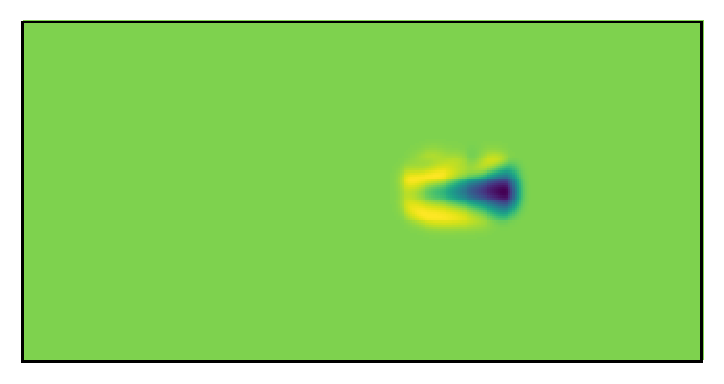
\includegraphics[width=\textwidth]{img/el_nino_mode.pdf}
%\end{subfigure}\hfill
\begin{subfigure}{.45\textwidth}\centering
    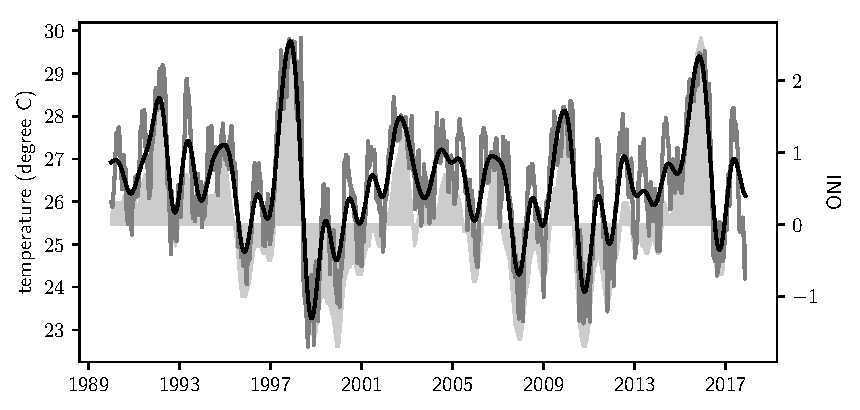
\includegraphics[width=\textwidth]{img/el_nino_filtered.pdf}
    \caption{temperature at (90,245) (dark grey), filtered temperature (black) ONI data (light grey fill)}
\end{subfigure}\hfill
\begin{subfigure}{.45\textwidth}\centering
    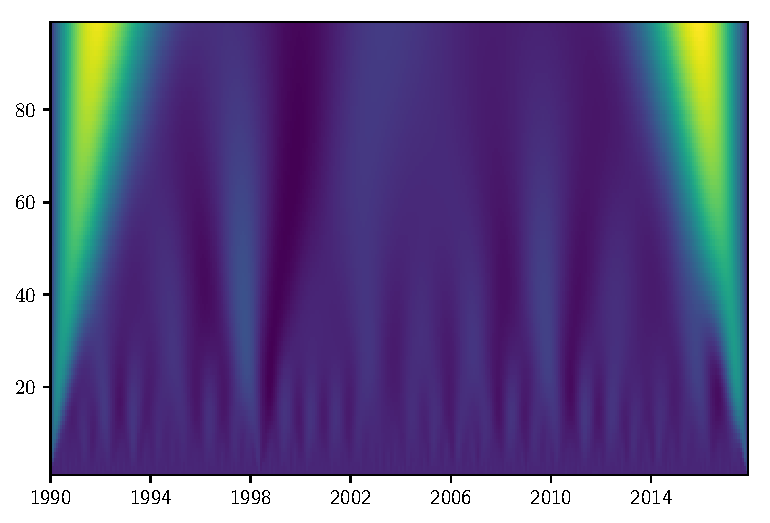
\includegraphics[width=\textwidth]{img/el_nino_wavelet_transform.pdf}
    \caption{CWT of temperature at (90,245) (ricker wavelet)}
\end{subfigure}
\caption{Analysis of temperature at (90,245)}
\label{elnino}
\end{figure}

\subsection{Prediction}
We train a neural net to predict the next time the ONI will be above a fixed threshold. To build the target data we first detect when the ONI reaches the specified threshold. These points are marked, and then the time to reach the next one of these points is found for each time in the given data set. We then train a neural network with the input being the current global ocean temperatures and the output being the next time until the ONI reaches the specified threshold using 5\% of the data for cross validation.

As before, since we do not have much time to train a network, and since we do not understand how to pick the proper network architecture, our results are not notable. That said everything we did was designed to be easily scaleable so that it could be adjusted in the future. This seems like an example of where a convolutional neural net might be useful.

\section{Summary and Conclusions}

The Discrete Wavelet Transform seems to provide a clean way of detecting and analyzing multi-scale phenomena without and sort of supervision. Given more time we would like to write an efficient algorithm to compute this transform. At the very least rather than projecting using inner products, slicing could be use for some wavelets. This would be more efficient in terms of floating point operations, and given fast memory access might prove feasible on our computing resources. Alternatively, and perhaps more practically , the algorithm could be implemented for parallel computation. Projecting onto a basis amounts to computing many independent inner products, which is the perfect type of problem for a GPU or large cluster. Parallelization would allow the fast computation of the projection onto any basis.

The Oceanic Ni\~no Index seems to be almost completely recoverable from a single point. This suggests that the definition of the index could be tightened. However, perhaps taking recordings over a larger area gives more precision.

Finally, we train a neural net to predict the next time the ONI will reach a certain threshold. Due to the limited time this was not very successful. However, our code is easily scaleable if we were to have more time to invest in the project.


\bibliographystyle{plain}
\bibliography{hw3}

\onecolumn
\section{Appendix A}
\label{AppendixA}
\lstinputlisting[linerange=\#<start:generate_wavelets>-\#<end:generate_wavelets>]{wavelettest.py}
\lstinputlisting[linerange=\#<start:svd_slice>-\#<end:svd_slice>]{hw3.py}

%\pagebreak
\section{Appendix B}
\lstinputlisting[linerange=\#<start:wavelet_decomp>-\#<end:wavelet_decomp>]{wavelettest.py}
\lstinputlisting[]{hw3.py}



\end{document}
